\documentclass[11pt,oneside,letterpaper]{article}

% graphicx package, useful for including eps and pdf graphics
\usepackage{graphicx}
\DeclareGraphicsExtensions{.pdf,.png,.jpg}

% basic packages
\usepackage{color} 
\usepackage{parskip}
\usepackage{float}

% text layout
\usepackage{geometry}
\geometry{textwidth=15cm} % 15.25cm for single-space, 16.25cm for double-space
\geometry{textheight=22cm} % 22cm for single-space, 22.5cm for double-space

% helps to keep figures from being orphaned on a page by themselves
\renewcommand{\topfraction}{0.85}
\renewcommand{\textfraction}{0.1}

% bold the 'Figure #' in the caption and separate it with a period
% Captions will be left justified
\usepackage[labelfont=bf,labelsep=period,font=small]{caption}

% review layout with double-spacing
%\usepackage{setspace} 
%\doublespacing
%\captionsetup{labelfont=bf,labelsep=period,font=doublespacing}

% cite package, to clean up citations in the main text. Do not remove.
\usepackage{cite}
%\renewcommand\citeleft{(}
%\renewcommand\citeright{)}
%\renewcommand\citeform[1]{\textsl{#1}}

% Remove brackets from numbering in list of References
\renewcommand\refname{\large References}
\makeatletter
\renewcommand{\@biblabel}[1]{\quad#1.}
\makeatother

\usepackage{authblk}
\renewcommand\Authands{ \& }
\renewcommand\Authfont{\normalsize \bf}
\renewcommand\Affilfont{\small \normalfont}

% notation
\usepackage{amsmath}
\usepackage{amssymb}
\newcommand{\point}{f_{\scriptscriptstyle \vert}}	% point likelihood
\newcommand{\threshold}{f_{\textstyle \lrcorner}}	% threshold likelihood
\newcommand{\interval}{f_{\sqcup}}					% interval likelihood
\newcommand{\mdssd}{\varphi}						% MDS standard deviation
\newcommand{\diffusionsd}{\sigma}					% Diffusion standard deviation
\newcommand{\driftsd}{\vartheta}					% Drift prior standard deviation
\newcommand{\tree}{\tau}							% Phylogeny
\newcommand{\vn}{n}									% Number of viruses
\newcommand{\sn}{k}									% Number of sera
\setlength{\arraycolsep}{2pt}
\newcommand{\twomatrix}[2]{\scriptsize \Big( \begin{matrix} #1 \\ #2 \end{matrix} \Big)}				% pretty inline matrix 
\newcommand{\fourmatrix}[4]{\scriptsize \Big( \begin{matrix} #1 & #2 \\ #3 & #4 \end{matrix} \Big)}		% pretty inline matrix 

% comments
\usepackage{ulem}
\definecolor{purple}{rgb}{0.459,0.109,0.538}
\def\tb#1#2{\sout{#1} \textcolor{purple}{#2}} 
\def\tbc#1{\textcolor{purple}{[#1]}}

%%% TITLE %%%
\title{\vspace{1.0cm} \LARGE \bf Revealing the competitive dynamics of influenza viruses through evolutionary cartography}

\author[1]{Trevor Bedford}
\author[2,3,4]{Marc A. Suchard}
\author[5]{Philippe Lemey}
\author[1]{Gytis Dudas}
\author[6]{Colin Russell}
\author[6,7]{Derek Smith}
\author[1,8]{Andrew Rambaut}

\affil[1]{Institute of Evolutionary Biology, University of Edinburgh, Edinburgh, UK}
\affil[2]{Department of Biomathematics, David Geffen School of Medicine at UCLA, University of California, Los Angeles CA, USA}
\affil[3]{Department of Human Genetics, David Geffen School of Medicine at UCLA, University of California, Los Angeles CA, USA}
\affil[4]{Department of Biostatistics, UCLA School of Public Health, University of California, Los Angeles CA, USA}
\affil[5]{Department of Microbiology and Immunology, Katholieke Universiteit Leuven, Leuven, Belgium}
\affil[6]{Department of Zoology, University of Cambridge, Cambridge, UK.}
\affil[7]{Department of Virology, Erasmus Medical Centre, Rotterdam, Netherlands.}
\affil[8]{Fogarty International Center, National Institutes of Health, Bethesda, MD, USA.}

\date{}

\begin{document}

\maketitle

%%% ABSTRACT %%%
\section*{Abstract}

Influenza viruses undergo continual antigenic evolution allowing mutant viruses to evade immunity acquired by the host population to previous virus strains.
However, the extent to which antigenic evolution determines competitive dynamics within and between virus clades A/H3N2, A/H1N1, B/Victoria and B/Yamagata has remained unclear.
Here, we develop a novel cartographic approach to simultaneously characterize the genetic and antigenic evolution of viral lineages.
Through this approach, we determine historical rates and patterns of antigenic drift in all four viral clades and we show that antigenic drift influences year-to-year variability in clade dominance.
We investigate the selective underpinnings for differing antigenic dynamics across clades and suggest that pleiotropic effects linked to antigenic mutation determine selective outcomes. 

%%% INTRODUCTION %%%
\section*{Introduction}

Seasonal influenza infects between 10\% and 20\% of the human population every year, causing 250,000 to 500,000 deaths annually \cite{flufactsheet}. 
While individuals develop long-lasting immunity to particular influenza strains after infection, antigenic mutations to the influenza virus genome result in proteins that are recognized to a lesser degree by the human immune system, leaving individuals susceptible to future infection. 
The influenza virus population continually evolves in antigenic phenotype in a process known as antigenic drift. 
A large proportion of the disease burden of influenza stems from antigenic drift; it is why vaccines remain only transiently effective. 
A thorough understanding of the process of antigenic drift is essential to our efforts to control mortality and morbidity through the use of a seasonal influenza vaccine.

Before 2009, there were four major clades of influenza circulating within the human population: A/H3N2, A/H1N1, B/Victoria and B/Yamagata. 
In the case of influenza A, subtypes A/H3N2 and A/H1N1 refer to the genes, hemagglutinin (H or HA) and neuraminidase (N or NA), that are primarily responsible for the antigenic character of a strain. 
In the case of influenza B, B/Vic and B/Yam refer to antigenically distinct lineages which diverged from one prior to 1980 \cite{Rota92}.
Mutations to the HA1 region of the hemagglutinin protein are thought to drive the majority of antigenic drift in the influenza virus \cite{Nelson07NatRevGenet}. 
Experimental characterization of antigenic phenotype is possible through the hemagglutination inhibition (HI) assay \cite{Hirst43}, which measures the cross-reactivity of one virus strain to serum raised against another strain through challenge or vaccination. 
Sera from older strains react poorly with more evolved viruses resulting in new strains having a transmission advantage over previously established strains.
HI assays have shown there to be little to no cross-reactivity between influenza clades A/H3N2, A/H1N1, B/Vic and B/Yam \cite{Hay01}.

The results of many HI assays across a multitude of virus strains can be combined to yield a two-dimensional map, quantifying antigenic similarity and distance \cite{Smith04}. 
The antigenic map of influenza A/H3N2 has shown largely linear movement of the influenza virus population since its introduction in 1968. 
Evolution of antigenic phenotype appears punctuated with periods of stasis interspersed by periods of more rapid innovation, while genetic evolution appears more continuous \cite{Smith04}, suggesting that a relatively small number of genetic changes or combinations of genetic changes may drive changes in antigenic phenotype. 
The process of antigenic drift results in the rapid turnover of the virus population. 
Although mutation occurs rapidly, standing genetic diversity is low and phylogenetic analysis shows a characteristically `spindly' tree with a single predominant trunk lineage and transitory side branches that persist for only 1--5 years \cite{Fitch97}.

Previously, the antigenic and genetic patterns of influenza evolution have been analyzed essentially in isolation. 
An antigenic map is constructed from a panel of HI measurements, and a phylogenetic tree is constructed from sequence data. 
However, the opportunity for a combined approach exists as both the antigenic map and the phylogenetic tree often contain many of the same isolates. 
Here, we implement a flexible Bayesian approach to jointly characterize the antigenic and genetic evolution of the influenza virus population. 
We apply this approach to investigate the dynamics of clades A/H3N2, A/H1N1, B/Vic and B/Yam. 

%%% RESULTS %%%
\section*{Results and Discussion}

\subsection*{Antigenic and evolutionary cartography}

In order to assess patterns of antigenic evolution among influenza strains, we implemented a Bayesian probabilistic analog of multidimensional scaling (MDS), referred to here as BMDS (see Methods).
In this model, viruses and sera are given $N$-dimensional locations, thus specifying an `antigenic map', such that distances between viruses and sera in this space are inversely proportional to cross-reactivity.
In the BMDS model, a map distance of one antigenic unit translates to an expectation of a 2-fold drop in HI titer between virus and sera.
Maps that produce pairwise distances most congruent with the observed titers will have a high likelihood and will be favored by the BMDS model.
We integrate over sources of uncertainty, such as antigenic locations, in a flexible Bayesian fashion.
We apply this model to HI measurements of virus isolates against post-infection ferret sera for influenza A/H3N2, A/H1N1, B/Vic and B/Yam (see Methods).

We test model performance by constructing a training dataset representing 90\% of the HI measurements of the A/H3N2 dataset and a test dataset representing the remaining 10\% of the full dataset. 
By fitting the BMDS model to the training dataset, we are able to predict HI titers in the test dataset and compare these predicted titers to observed titers in the test dataset. 
We find that a BMDS analog of the model used by Smith et al.\ \cite{Smith04}, in which viruses and sera are represented as 2D locations and expected titer is relative to the maximum titer of a particular ferret serum, performs well, yielding an average absolute predictive error of 0.87 log$_2$ HI titers (Table \ref{errortable}).
We find that a model with two dimensional antigenic locations predicts test data to the same precision as a 3D model, but performs substantially better than a 1D model or models with four or more dimensions (Table \ref{errortable}), and thus specify a two dimensional model in all subsequent analyses.
We extend this model by estimating the strength of overall reactivity of each serum rather than fixing this at the maximum titer, and additionally, by estimating the strength of reactivity of each virus isolate.
We refer to these estimates as serum effects and virus effects, respectively.
We find that including these effects decreases test error to 0.75 for influenza A/H3N2.
We arrive at similar precisions when repeating this analysis for A/H1N1, B/Vic and B/Yam.
For the 2D model with serum and virus effects, A/H1N1 shows a test error of 0.64, B/Vic shows a test error of 0.74 and B/Yam shows a test error of 0.80.

%%% errortable %%%
\begin{table}[h]
	\centering
	\caption{\textbf{Absolute prediction error of log$_2$ HI titer against A/H3N2 test data across models.}}
	\label{errortable}		
	\begin{tabular}{ c c c c c } 
	\hline
	BMDS dimension 	& 	Serum effects 	&	Virus effects	& 	Test error	\\
	\hline	
	1D 				&	Fixed 			&	None			&	1.05		\\	
	2D 				&	Fixed 			&	None			&	0.87 		\\
	3D 				&	Fixed 			&	None			&	0.87		\\
	4D 				&	Fixed 			&	None			&	0.91		\\
	5D 				&	Fixed 			&	None			&	0.97		\\	
	2D 				&	Estimated 		&	None			&	0.78		\\	
	2D 				&	Estimated 		&	Estimated		&	0.75		\\		
	\hline
	\end{tabular}
\end{table}

Previous work on influenza antigenic and genetic evolution has examined antigenic and genetic patterns in isolation, and then compared the results to assess congruence of these two aspects of evolution \cite{Hay01,Smith04,Russell08}. 
Here, we simultaneously model antigenic and genetic evolution by adopting an evolutionary diffusion process \cite{Lemey10}, wherein a virus's antigenic character state evolves along branches of phylogenetic tree according to Brownian motion process (see Methods).
The diffusion process acts as a prior, so that genetically similar viruses are expected to have antigenic locations that lie close to one another, and thus we model the relationship between genetic change and accrual of antigenic distance.
We include sequence data for A/H3N2, A/H1N1, B/Vic and B/Yam to estimate this diffusion process.
We find similar levels of predictive accuracy when including the diffusion process with A/H3N2 showing a test error of 0.75, A/H1N1 showing a test error of 0.66, B/Vic showing a test error of 0.70 and B/Yam showing a test error of 0.78.

\subsection*{Antigenic evolution across influenza lineages}

Through our analysis, we reveal the evolutionary basis for antigenic phenotype in influenza A/H3N2, A/H1N1, B/Vic and B/Yam (Figure~\ref{map}).
Over the time period of 1968 to 2011, influenza A/H3N2 shows substantially more antigenic evolution than is exhibited by A/H1N1 over the course of 1977 to 2009 or B/Vic and B/Yam over the course of 1986 to 2011.
We observe prominent antigenic clusters in A/H3N2 and A/H1N1, but less obvious clustering in B/Vic and B/Yam.
Antigenic clusters show high genetic similarity, so that we only observe a single diffusion event leading to each cluster, rather than the repeated emergence of clusters.
This analysis makes the fate of antigenic clusters obvious, with two clusters in A/H3N2 (Texas/77 and Beijing/89) appearing to be evolutionary dead-ends.

%%% map %%%
\begin{figure}[h]
	\centering		
	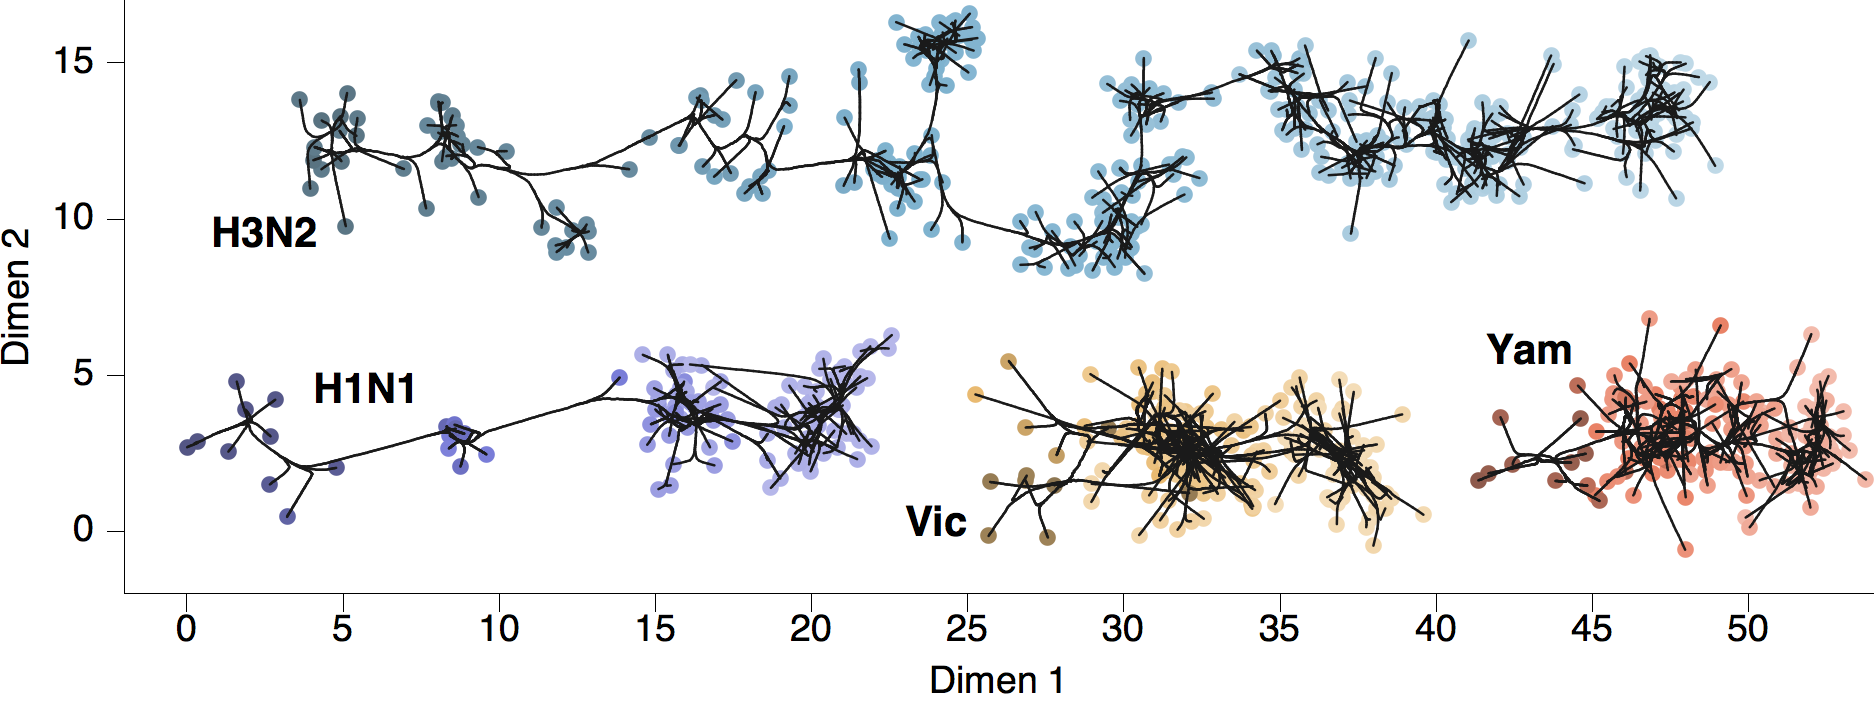
\includegraphics[width=0.95\textwidth]{figures/map}
	\caption{\textbf{Antigenic locations of A/H3N2, A/H1N1, B/Vic and B/Yam viruses showing evolutionary relationships between virus samples.} 
	Circles represent a posterior sample of virus locations and have been colored based on year of isolation in 4-year intervals.
	Antigenic units represent two-fold dilutions of the HI assay.
	Distances between clades, e.g.\ A/H3N2 and A/H1N1, are arbitrary.
	Lines represent mean posterior diffusion paths when virus locations are fixed.} 
	\label{map} 
\end{figure}

HI assays lack sensitivity beyond a certain point, so that for A/H3N2, cross-reactive measurements only exist between strains sampled at most 11 years apart, leaving only threshold titers, e.g.\ `$<$40', in more temporally distant comparisons.  
Because of the threshold of sensitivity of the HI assay, it's impossible to distinguish a linear trajectory in 2D antigenic space, from a somewhat curved trajectory, so long as the curve does not bring antigenic phenotype full circle to have cross-reactive measurements between temporally distant strains.
To solve this problem of identifiability, we assumed a weak prior that favors linear movement in the 2D antigenic space, with the slope of the linear relationship and the precision of the relationship incorporated into the Bayesian model (see Methods).
Incorporating this prior made no difference in predictive ability of the model; test error for A/H3N2 was 0.75 log$_2$ HI titers whether the prior was included or excluded.
Because of this, we interpret antigenic locations locally rather than globally.
We can determine the rate of antigenic movement of virus lineages without knowing the larger configuration that the movement occurs under.
 
We find that influenza A/H3N2 evolved along antigenic dimension 1 at a rate of 1.00 antigenic units per year, with a 95\% highest posterior density (HPD) interval of 0.97--1.04 (Figure~\ref{drift}).
However, we observe occasional large jumps in antigenic phenotype (Figure~\ref{drift}), corresponding to cluster transitions identified by Smith et al. \cite{Smith04}.  
Most variation is contained within the first antigenic dimension, but dimension 2 occasionally shows variation when two antigenically distinct lineages emerge and transiently coexist (Figure~\ref{map}), as is the case with the previously identified Beijing/89 and Beijing/92 clusters.

%%% drift %%%
\begin{figure}[h]
	\centering		
	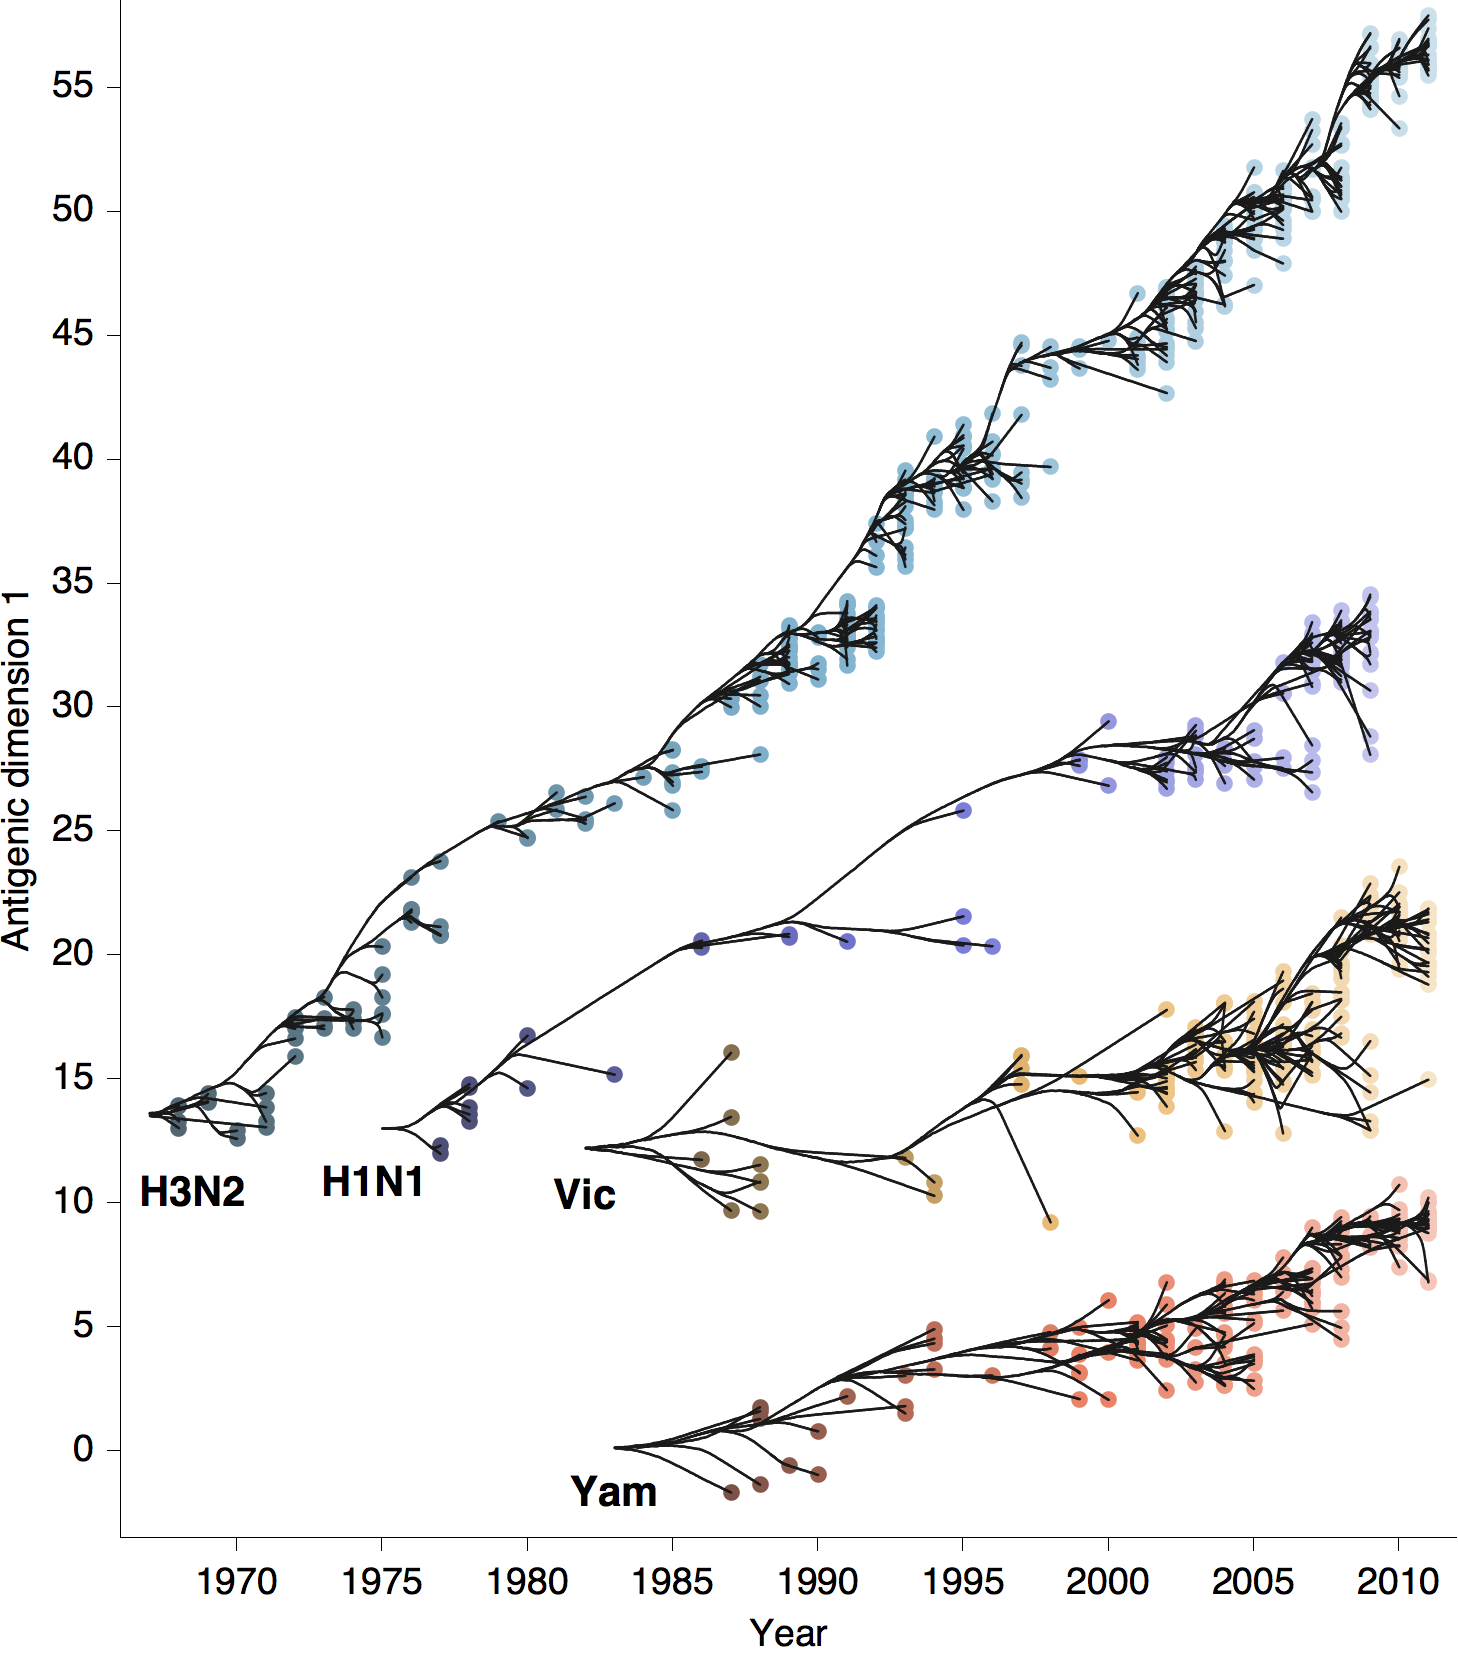
\includegraphics[width=0.75\textwidth]{figures/drift}
	\caption{\textbf{Antigenic drift of A/H3N2, A/H1N1, B/Vic and B/Yam viruses showing evolutionary relationships between virus samples.} 
	Antigenic drift is shown in terms of change of location in the first antigenic dimension through time.
	Circles represent a posterior sample of virus locations and have been colored based on year of isolation in 4-year intervals.
	Antigenic units represent two-fold dilutions of the HI assay.
	Distances between clades, e.g.\ A/H3N2 and A/H1N1, are arbitrary.
	Lines represent mean posterior diffusion paths when virus locations are fixed.} 
	\label{drift} 
\end{figure}

We find that other clades of influenza evolved in antigenic phenotype substantially slower than A/H3N2 (Figure~\ref{drift}).
Influenza A/H1N1 evolved at a rate of 0.55 units per year (HPD 0.49--0.62), but showing a similar pattern of punctuated antigenic evolution with occasional larger jumps in phenotype, such as the emergence of the Solomon Islands/06 cluster.  
Influenza B/Victoria also evolved relatively slowly, with an average rates of 0.41 (HPD 0.29--0.55) units per year.
Influenza B/Vic appears to show some degree of punctuated antigenic evolution with a recent transition creating the Brisbane/08 cluster.
Interestingly, a minor lineage of B/Vic has persisted, which rather than moving forward in antigenic dimension 1 has moved down in antigenic dimension 2 (Figure~\ref{map}, Figure~\ref{drift}).
The eventual fate of this lineage has yet to be determined.
Influenza B/Yamagata evolved slower still, with an average rate of and 0.21 (HPD 0.10--0.28) units per year.
Very little punctuated evolution is apparent in the evolution of B/Yam.

Interestingly, although antigenic clusters seem to emerge in a punctuated fashion in influenza A/H3N2, year-to-year antigenic drift relatively constant through time with most years exhibiting an intermediate level of drift (Figure~\ref{jumps}).
We calculate year-to-year antigenic drift for years 1992 to 2011 by calculating the average location along dimension 1 of phylogenetic lineages present at year $i$ and comparing this location to the average location of phylogenetic lineages present at year $i-1$.
For A/H3N2, the largest cluster transition we observe is the emergence of the Sydney/97 cluster in 1997, evident as a large gap in virus locations along dimension 1 in Figure~\ref{drift}.
However, in 1997 only three of the nine viruses sampled show the Sydney/97 phenotype, while the remaining six viruses exhibit the old Wuhan/95 phenotype.
In 1998, three of the four viruses sampled show the Sydney/97 phenotype, with the remaining virus still showing the Wuhan/95 phenotype.
In 1999, all sampled viruses exhibit the Sydney/97 phenotype.
Thus, we observe nearly equal rates of year-to-year antigenic drift in mean phenotype in going from 1996 to 1997, from 1997 to 1998 and from 1998 to 1999, rather than an immediate jump in mean antigenic phenotype in 1997 (Figure~\ref{jumps}).
However, once the transition is completed in 1999, year-to-year antigenic drift drops, showing very low values in 2000 and 2001 before the Fujian/02 variant emerges.
In addition to showing greater overall rates of antigenic drift, A/H3N2 shows greater variation in year-to-year drift than seen in A/H1N1 or influenza B (Figure~\ref{jumps}).
We find that the standard deviation in year-to-year drift is 0.80 antigenic units for A/H3N2, 0.38 units for A/H1N1, 0.44 units for B/Vic and 0.19 units for B/Yam.

%%% jumps %%%
\begin{figure}[h]
	\centering		
	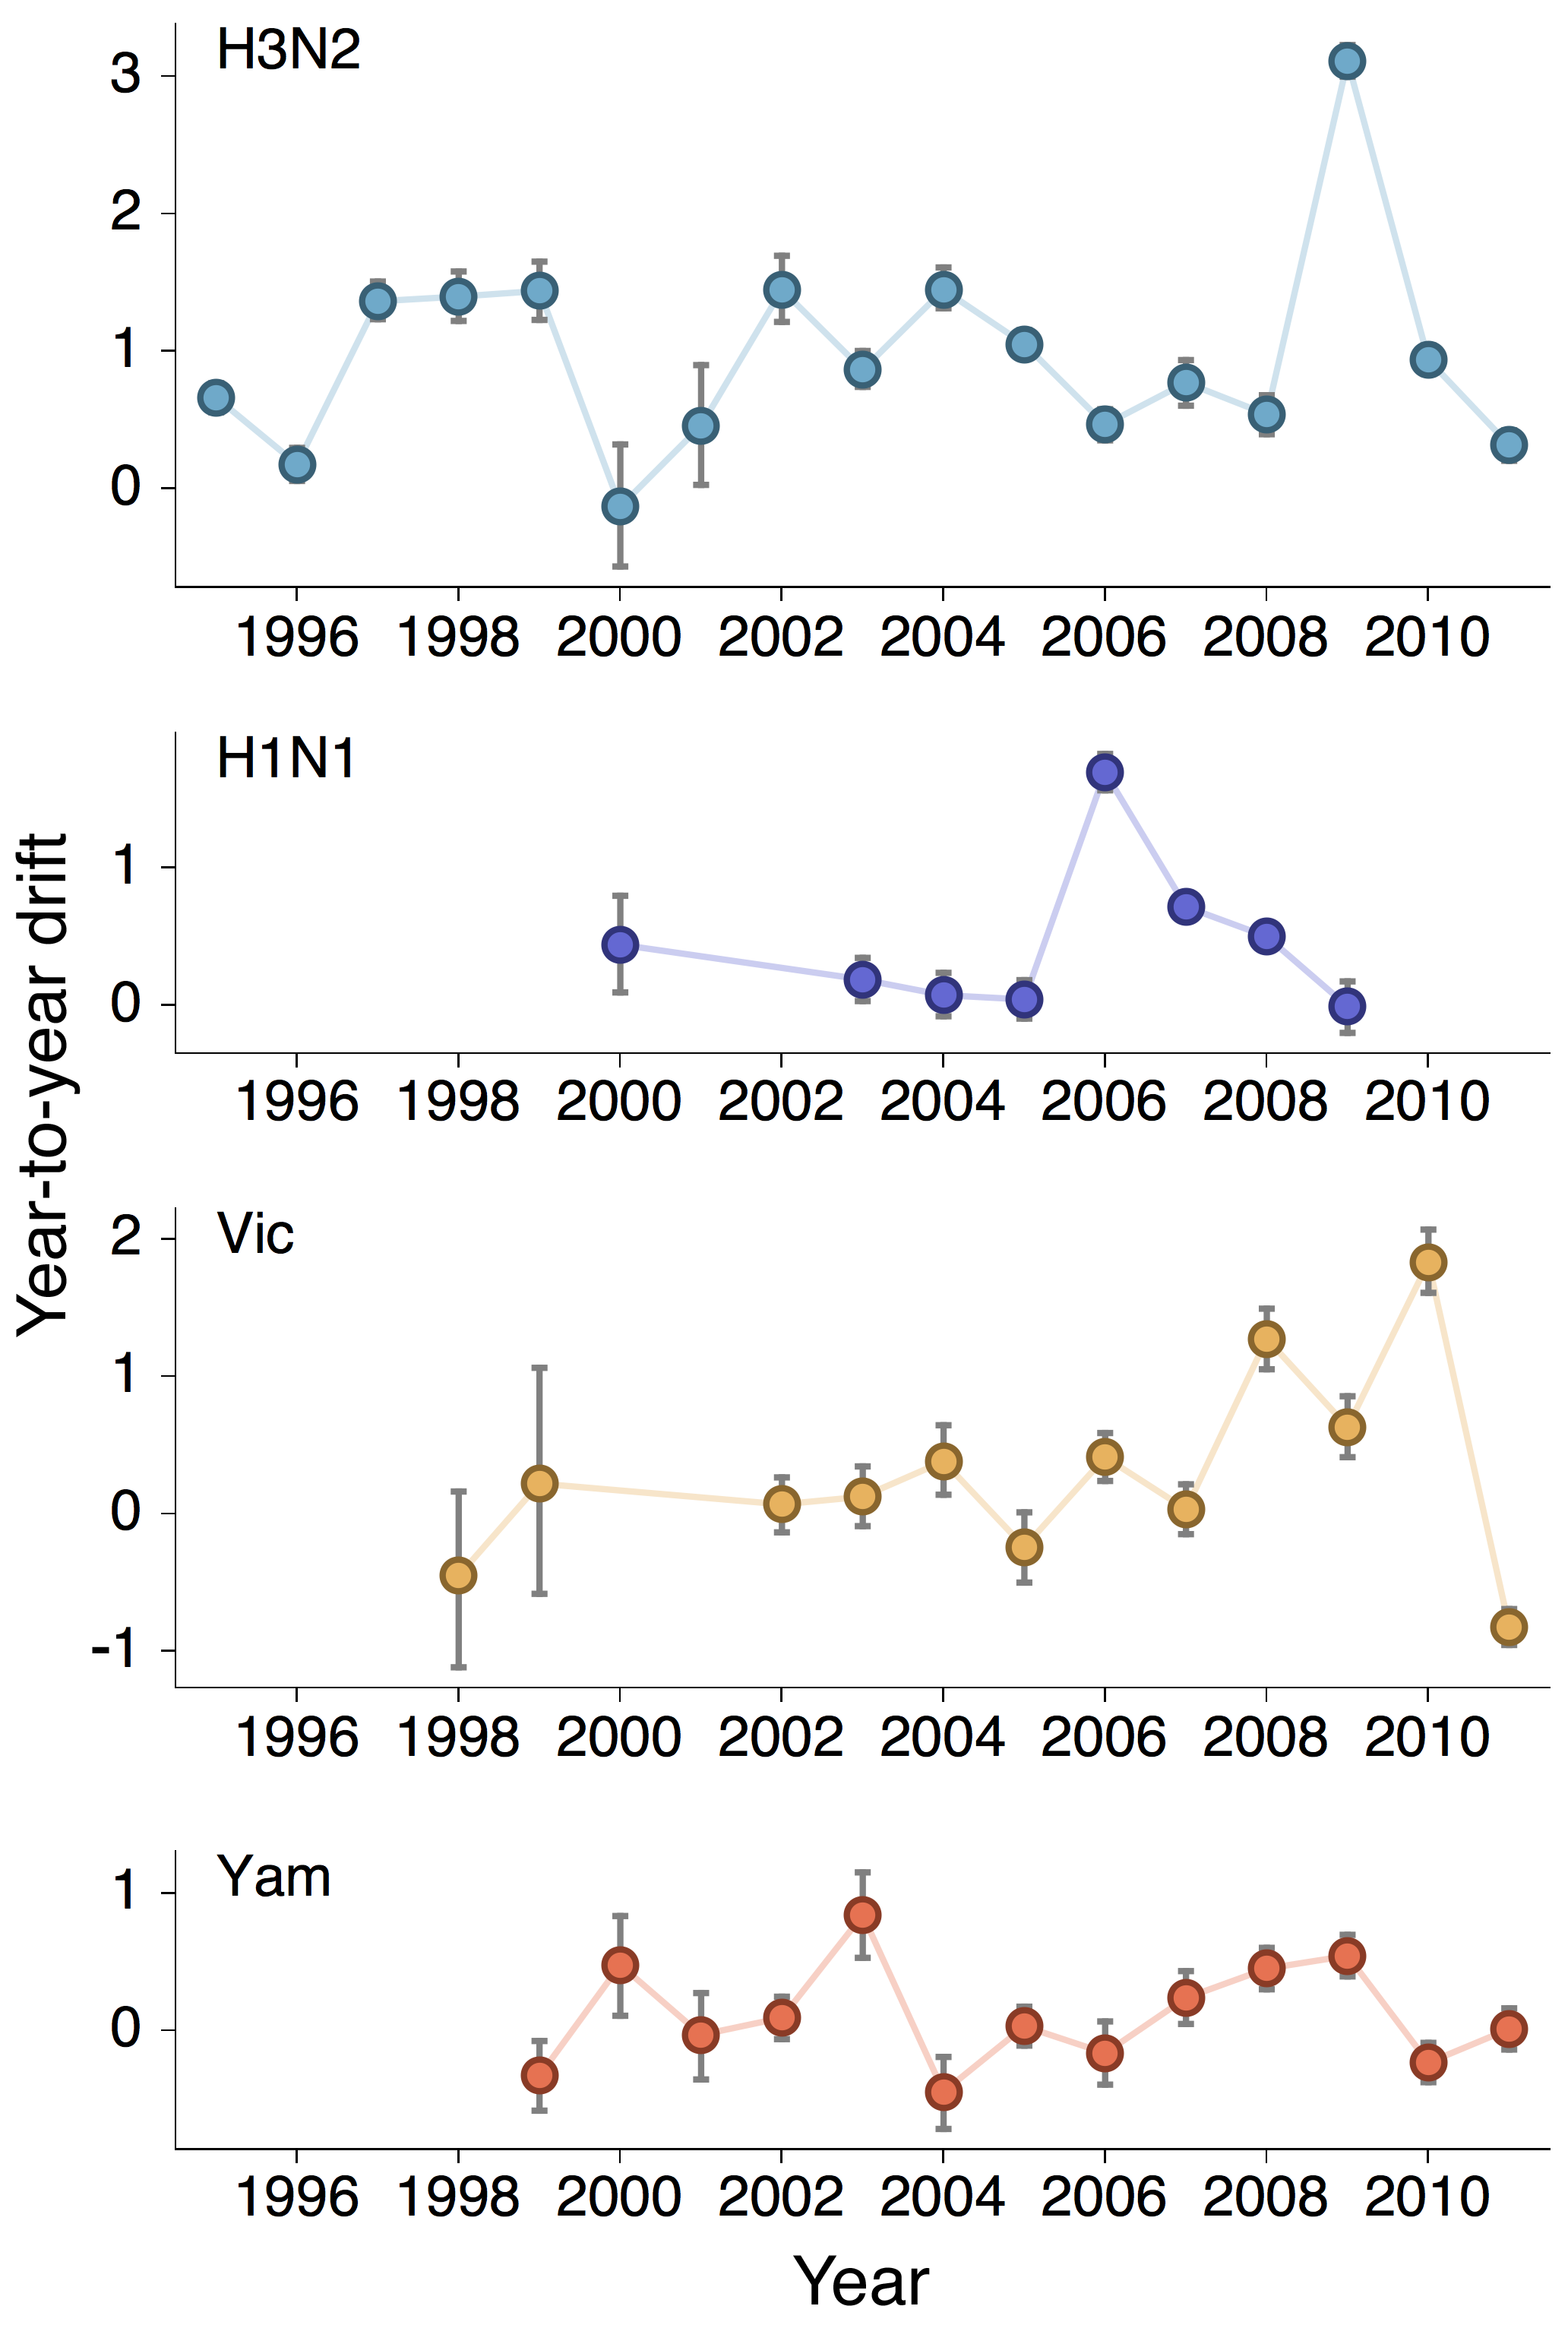
\includegraphics[width=0.85\textwidth]{figures/jumps}
	\caption{\textbf{Year-to-year antigenic drift between 1992 and 2011 of A/H3N2, A/H1N1, B/Vic and B/Yam viruses.} 
	(A) Histograms of year-to-year antigenic drift across influenza clades.
	(B) Timeseries of year-to-year antigenic drift across influenza clades from 1992 to 2011.
	Year-to-year antigenic drift for a virus clade for year $i$ is measured as the mean of antigenic dimension 1 of phylogenetic lineages in year $i$ compared to the mean of antigenic dimension 1 of phylogenetic lineages from the previous year $i-1$.
	For example, 2000 signifies difference in antigenic dimension 1 between 1999 and 2000.
	} 
	\label{jumps} 
\end{figure}

\subsection*{Epidemiological consequences of antigenic drift}

We investigated the relative rates of antigenic evolution in A/H3N2, A/H1N1, B/Vic and B/Yam from 1998 to 2010, finding a general correspondence between antigenic drift in dimension 1 and relative incidence within each influenza clade (Figure~\ref{incidence}).
Here, we take the measurements of year-to-year antigenic drift from the preceding section (Figure~\ref{jumps}) and calculate the relative contribution to total antigenic drift for each clade in each year.
We compare these measurements of relative antigenic drift to relative isolations of viruses form each clade in the USA from 1998 to 2011 (see Methods).
From 1998 to 2010, A/H3N2 accounted for the majority of antigenic drift (56\%), while A/H1N1, B/Vic and B/Yam split the remainder, accounting for 15\%, 21\% and 7\%, respectively.
Similarly, A/H3N2 was responsible for the majority of incidence (56\%) during this time period.
Influenza A/H1N1 accounted for 20\% of incidence, B/Vic accounted for 13\% of incidence and B/Yam accounted for 11\% of incidence.
These proportions are significantly similar to one another (randomization test, $p = 0.011$).

%%% incidence %%%
\begin{figure}[tb]
	\centering		
	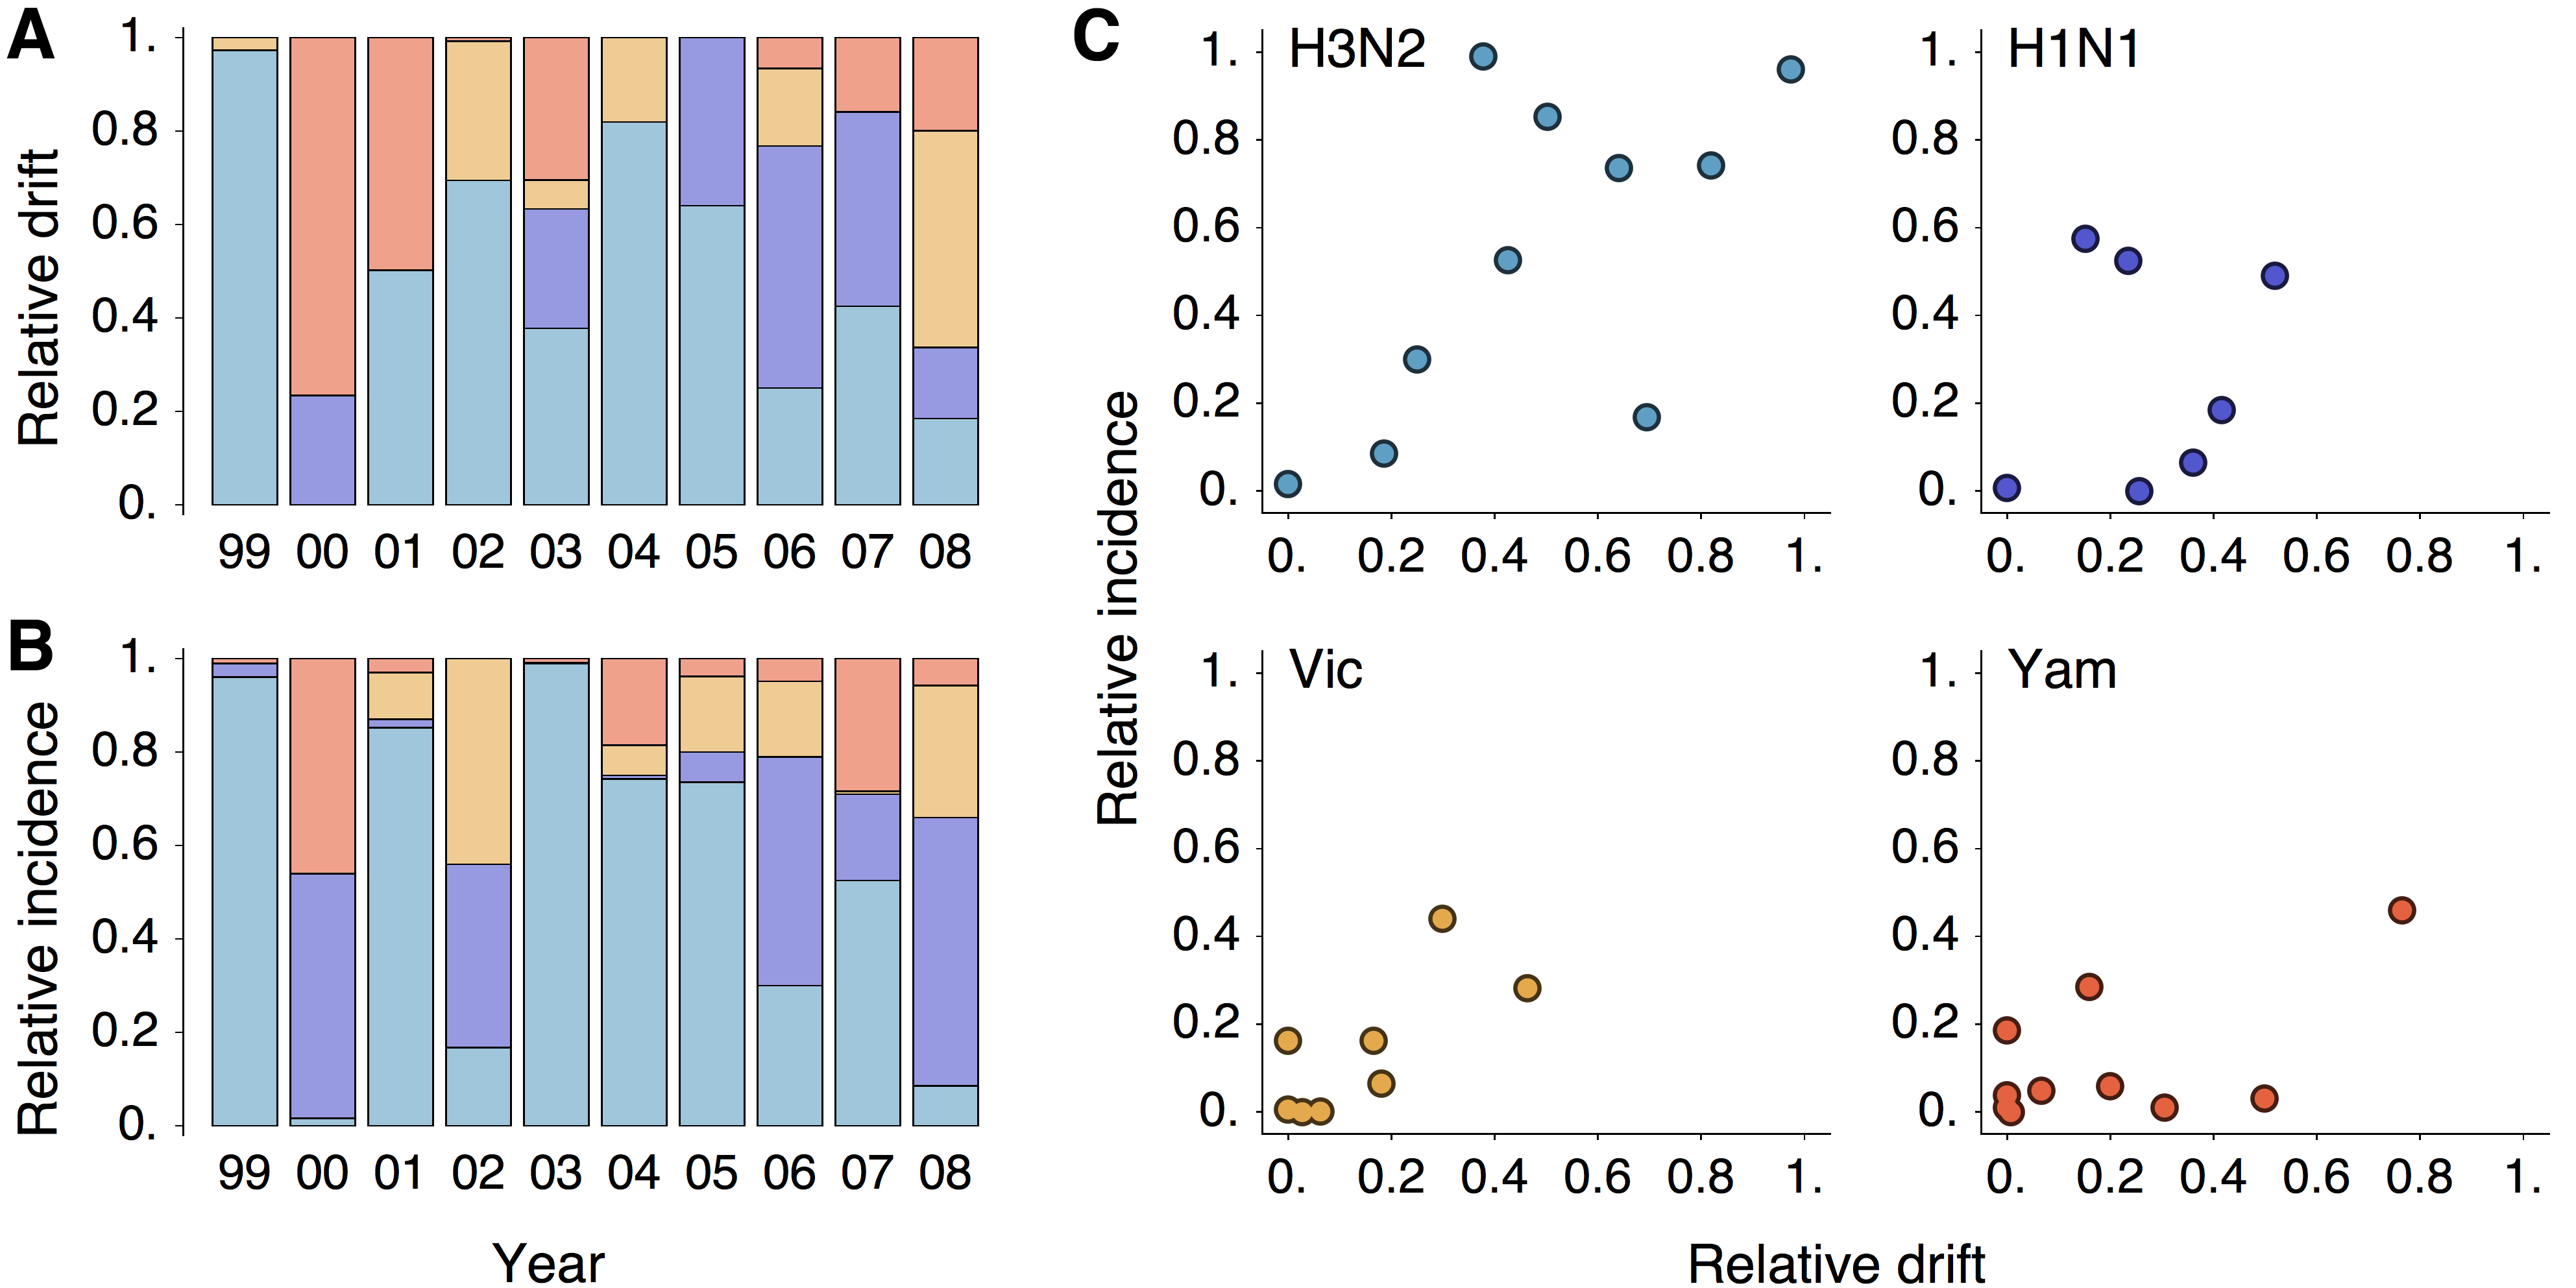
\includegraphics[width=0.95\textwidth]{figures/incidence}
	\caption{\textbf{Relative antigenic drift and relative incidence of A/H3N2, A/H1N1, B/Vic and B/Yam from 1999 to 2008.} 
	(A) Relative antigenic drift of influenza clades.
	Relative antigenic drift for A/H3N2 is measured as the drift of A/H3N2 viruses divided by the sum of drift for A/H3N2, A/H1N1, B/Vic and B/Yam.
	For example, `00' signifies difference in antigenic dimension 1 between 1999 and 2000.
	Years with negative absolute drift were assigned a relative antigenic drift of 0.
	(B) Relative incidence of influenza clades determined through relative isolation counts in the USA for winter influenza seasons.
	Here, `99' refers to the 1999/2000 influenza season.
	(C) Correlation of relative antigenic drift and relative incidence in each influenza clade.
	Scatterplots represent drift from year $i-1$ to year $i$ compared to incidence in winter season beginning in year $i$, e.g. drift from 1998 to 1999 compared to incidence in the 1999/2000 influenza season.
	} 
	\label{incidence} 
\end{figure}

Additionally, year-to-year comparisons show a similar pattern (Figure~\ref{incidence}). 
Here, we define antigenic drift from year $i-1$ to year $i$ as the difference between the average location in dimension 1 of viruses sampled in year $i-1$ and the average location in dimension 1 of viruses sampled in year $i$.
For example, we find that every year that A/H3N2 is responsible for the majority of antigenic drift (1998, 1998, 2001, 2002, 2003, 2004, 2005, 2009) shows A/H3N2 as dominating viral isolations.
Additionally, the two strongest years of A/H1N1 drift (2000 and 2006) are dominated by A/H1N1 over A/H3N2.
We find an overall correlation between clade-specific relative antigenic drift and clade-specific incidence of $r = 0.71$ (Pearson correlation, $p = 2.14 \times 10^{-9}$).
Correlation is present to greater of lesser degrees for each of the four clades, with $r_\mathrm{H3} = 0.57$, $r_\mathrm{H1} = 0.38$, $r_\mathrm{Vic} = 0.46$ and $r_\mathrm{Yam} = 0.40$.
Pandemic H1N1 is present in the incidence data in 2009 and afterwards, however, our estimates of relative incidence only include isolations of seasonal A/H3N2, A/H1N1, B/Vic and B/Yam.

These findings clearly demonstrate the epidemiological importance of antigenic drift and show that incidence of influenza clades A/H3N2, A/H1N1, B/Vic and B/Yam is strongly impacted by levels of antigenic drift within each clade.
Furthermore, these findings suggest that the composition of a particular influenza season could be estimated ahead of time by examining the degree of antigenic drift between influenza clades.
However, these findings alone do not conclusively show interference between clades; more work needs to be done to establish whether antigenic drift within one influenza clades drives down incidence in other clades.

\subsection*{Conversion of antigenic mutation into fixed differences}

We observe a faster rate of antigenic drift in influenza A/H3N2 than in A/H1N1 or influenza B.
Previous work using general epidemiological models has suggested that a greater rate of antigenic drift may emerge from either a greater fundamental reproductive number $R_0$ or a faster rate of mutation decreasing cross-immunity \cite{Gog02,Lin03}.
Owing to these and similar findings, subsequent work has ascribed differences in the evolution in A/H3N2 relative to A/H1N1 and influenza B to either greater $R_0$ or greater mutation rate \cite{Ferguson03,Bedford12}.

Here, we examine the conversion of newly acquired antigenic mutation into fixed differences by comparing rates of antigenic diffusion to the degree of persistence on phylogeny branches from A/H3N2, A/H1N1, B/Vic and B/Yam (Figure~\ref{accumulation}A).
Here, we observe that in all four clades new antigenic mutations, do not, on average, move antigenic dimension 1 forward or back, consistent with a model of antigenic mutations progressing in a random direction.
However, successful mutations that have persisted in the influenza population, tend to move the antigenic phenotype forward along dimension 1.
This result indicates that forward movement along antigenic dimension 1 is an advantageous trait and is promoted by natural selection \cite{Bedford12}.
The rate of diffusion of persistent lineages is substantially greater in A/H3N2 than in A/H1N1, B/Vic or B/Yam.
For A/H3N2 we see a two-year window during which mutations may be present on side branches of the phylogeny.
After two years, mutations lie along the trunk of the phylogeny and the rate at which the trunk lineage drifts along antigenic dimension 1 is equal to the overall rate at which the population drifts along dimension 1.

%%% accumulation %%%
\begin{figure}[tb]
	\centering		
	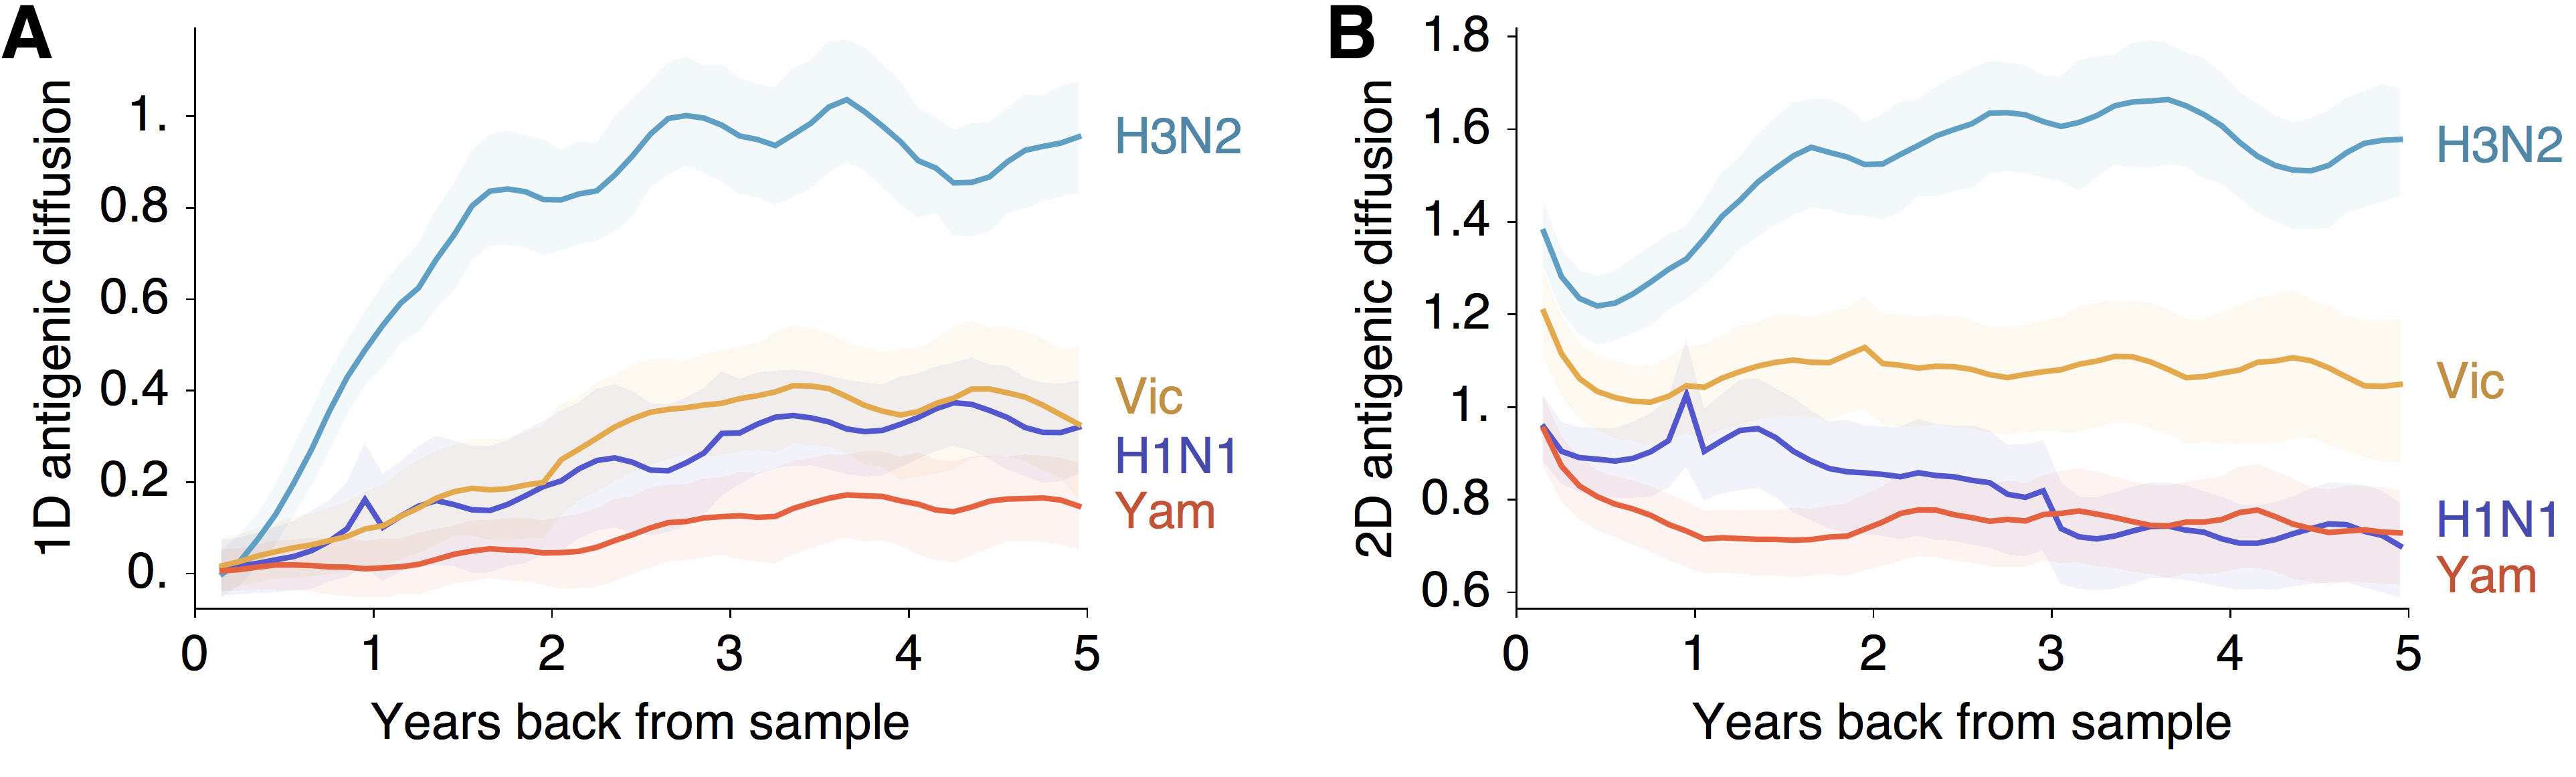
\includegraphics[width=0.95\textwidth]{figures/accumulation}
	\caption{\textbf{Rate of antigenic diffusion of influenza lineages categorized by time back from sampling.}
	(A) Rate of diffusion in terms of antigenic units per year only along antigenic dimension 1.
	(B) Rate of diffusion in terms of antigenic units per year along both antigenic dimensions 1 and 2.
	In the diffusion model, the antigenic location of each virus sample can be calculated back through time.
	Here, when the $x$-axis is 1, we show the rate of diffusion 1 year back from from the date of sampling averaged across all virus samples.
	When the $x$-axis is close to 0, the $y$-axis shows the rate of diffusion near tips of the phylogeny, and when the $x$-axis is large, the $y$-axis shows the rate of diffusion along the trunk of the phylogeny.
	} 
	\label{accumulation} 
\end{figure}

If we examine the introduction of new mutations in two dimensions, we see that A/H3N2 appears to mutate in antigenic phenotype more rapidly than B/Vic, which mutates more rapidly still than A/H1N1 or B/Yam (Figure~\ref{accumulation}B).
Thus, we have direct evidence that the rate of antigenic mutation is greater in A/H3N2 than in A/H1N1 or influenza B.
However, we observe an interesting additional effect.
The rate of diffusion of persistent lineages is greater than the rate of mutation in influenza A/H3N2, but smaller than the rate of mutation in A/H1N1, B/Vic and B/Yam.
This yields the surprising conclusion that although antigenic mutation in general is favored in A/H3N2, it is deleterious and opposed by natural selection in A/H1N1 and B.

We suggest that this finding could be due to the pleiotropic effects associated with antigenic change, in which antigenic mutations often result in other phenotypic effects, including decreased protein function \cite{Kaverin04,Rudneva12}.
Thus, we expect that many antigenic variants may be at inherent disadvantage against other strains, even though they benefit from a transmission advantage mediated by host immunity.
Because of this, some antigenic mutations, i.e.\ those that move forward along antigenic dimension 1, may be, on the whole, advantageous, while other antigenic mutations may be, on the whole, deleterious.
In this context, it is especially interesting that antigenic mutations appear to be, on the whole, more advantageous in A/H3N2.
It seems possible that the H3 protein may have fewer pleiotropic constraints that the the H1 protein or B hemagglutinin protein.
However, more work is necessary to investigate this hypothesis.

In this context, it is especially interesting that adaptive fixation in the HA1 protein determined through analysis of nonsynonymous and synonymous evolution is substantially greater in A/H3N2 than in A/H1N1 \cite{Wolf06, Bhatt11}.
Thus, we conclude that additional adaptive fixations at the amino acid level translate to greater rates of adaptive antigenic change. 

%%% CONCLUSIONS %%%
\section*{Conclusions}

In this study we provide a foundation for evolutionary antigenic cartography, which seeks to simultaneously assess antigenic phenotype and antigenic evolution.
We use this approach to characterize competitive dynamics across influenza clades A/H3N2, A/H1N1, B/Vic and B/Yam and show that antigenic evolution drives strain replacement in each influenza clade.
However, A/H3N2 shows substantially stronger signals of adaptive antigenic evolution, evolving faster in antigenic phenotype and showing more efficient conversion of transient antigenic polymorphism into fixed differences.
Correspondingly, we observe substantially greater levels of incidence in A/H3N2 than in other influenza clades.
We suggest that antigenic evolution strongly influences competitive dynamics both within and between influenza clades.

The statistical framework presented here represents a baseline to which further advancements in modeling antigenic phenotype and evolution may be made.
For example, our likelihood-based model facilities the inclusion of possible covariates affecting immunological titer, which could include experimental factors such as red blood cell type is used in the HI assay \cite{Lin12} and whether oseltamivir is included in the HI reaction \cite{Lin10}.
Additionally, this framework should be ideally suited to uncovering genetic determinants of antigenic change, as both the sequence state and antigenic location of internal nodes in the phylogeny may be estimated.
In this fashion, it should be possible to correlate sequence substitutions directly to antigenic diffusion.

Further work characterizing antigenic evolution in the human influenza virus may eventually prove to be crucial in improving vaccine strain selection.

%%% METHODS %%%
\section*{Methods}

\subsection*{Bayesian multidimensional scaling}

Antigenic characteristics of viral strains are often assessed through immunological assays such as the hemagglutination inhibition (HI) assay \cite{Hirst43}.  
At heart, these assays compare the reactivity of one virus strain to antibodies raised against another virus strain via challenge or vaccination.  
In the case of HI, the measurement of cross-reactivity takes the form of a titer $H_{ij}$ representing the dilution factor at which serum raised against virus $j$ ceases to be effective at inhibiting binding of virus $i$.  
These factors are commonly assessed by serial dilution, so that HI titers will form a log series, 40, 80, 160, etc \dots.
However, due to experimental constraints, most comparisons cannot be made, leading to a sparse observation matrix $\mathbf{H} = \{H_{ij}\}$.  
Further, measurements are usually interval and truncated, e.g.\ inhibition may cease somewhere between the serial titers of 160 and 320, or inhibition may be absent at all titers assayed, suggesting a threshold somewhere between 0 and 40.  

Previous work \cite{Smith04, Cai10} has used multidimensional scaling to place viruses and sera on an `antigenic map'.  
These methods heuristically optimize locations of viruses and sera by seeking to minimize the sum of squared errors between titers predicted by map locations and observed titers.  
Antigenic maps produced by these methods have proved useful in categorizing virus phenotypes \cite{Smith04}, but the extension of these methods to integrate genetic data has not yet been attained.

Here, we follow previous models in representing antigenic locations as points in an $N$-dimensional antigenic map. 
Our goal is to find an optimal projection of the high-dimensional distance matrix $\mathbf{H}$ into a lower number of dimensions. 
We conduct this projection using Bayesian multidimensional scaling (BMDS) \cite{Oh01} in which a probabilistic model is constructed to quantify the fit of a particular configuration of cartographic locations to the observed matrix of serological measurements.

Let $X_i \in \Re^{P}$ represent the cartographic location of virus $i$ for $i = 1,\ldots,\vn$, and $Y_j$ represent the cartographic location of serum $j$ for $j = 1,\ldots,\sn$.
Virus and serum may be isolated from / raised against the same strain and have different cartographic locations.
Typically, $P = 2$, but higher or lower dimensions may better reflect the data.  
This gives a set of distances between virus and serum cartographic locations 
\begin{equation}
	\delta_{ij} =  || X_i - Y_j ||_2.
\end{equation}
With $H_{ij}$ as the log$_2$ titer of virus $i$ against serum $j$, immunological distance can be defined as
\begin{equation}
	d_{ij} =  S_j - H_{ij},
\end{equation}
where $S_j = \max ( H_{1j},\ldots,H_{\vn j} )$.
Traditionally, the goal of multidimensional scaling (MDS) optimizes over $\mathbf{X}$ and $\mathbf{Y}$ such that
\begin{equation}
	\sum_{(i,j) \in \cal I} 
	\left(
		\delta_{ij} - d_{ij}
	\right)^2
\end{equation}
is minimized, where $\cal I = \{ (i,j) : H_{ij} \mbox{ is measured} \}$. 
Here, we instead assume a probabilistic interpretation in which an observed titer is normally distributed around its cartographic expectation
\begin{equation} \label{hij}
	H_{ij} \sim \mbox{TruncatedNormal}( S_j - \delta_{ij}, \mdssd^2 ),
\end{equation}
and the likelihood of observing a particular titer given the placement of antigenic locations is 
\begin{equation} 
	\point(H_{ij}) = \phi \left( \frac{ H_{ij} + \delta_{ij} - S_j }{ \mdssd } \right),
\end{equation}
where $\mdssd^2$ represents variance and $\phi(\cdot)$ represents the standard normal PDF.
HI assays sometimes show no inhibition at all measured titrations, e.g.\ a measurement can be reported as `$<$40'.
In this case, the likelihood of observing the threshold measurement follows the cumulative density of the lower tail of the normal distribution
\begin{equation} 
	\threshold(H_{ij}) = \Phi \left( \frac{ H_{ij} + \delta_{ij} - S_j }{ \mdssd } \right),
\end{equation}
where $\Phi(\cdot)$ represents the standard normal CDF.
Although it is simplest to assume that immunological measurements represent point estimates, it seems more natural to assume that the threshold for inhibition occurs between two titers, e.g.\ we observe inhibition at 1:40 dilution and no inhibition at 1:80 dilution.
Rather than taking the HI titer as 40, we can instead treat this as an interval measurement, assuming that the exact titer for inhibition would occur somewhere between 40 and 80.
HI titers are usually reported as the highest titer that successfully inhibits virus binding, so that in this case, we calculate the likelihood of an interval measurement as
\begin{equation} 
	\interval(H_{ij}) = \Phi \left( \frac{ H_{ij} + \delta_{ij} - S_j + 1 }{ \mdssd } \right) - \Phi \left( \frac{ H_{ij} + \delta_{ij} - S_j }{\mdssd} \right).
\end{equation}
These likelihoods are illustrated in Figure~\ref{hij_likelihood}.
Throughout our analyses, we use interval likelihoods $\interval$ rather than point likelihoods $\point$ unless otherwise noted.

%%% hij_likelihood %%%
\begin{figure}[tb]
	\centering		
	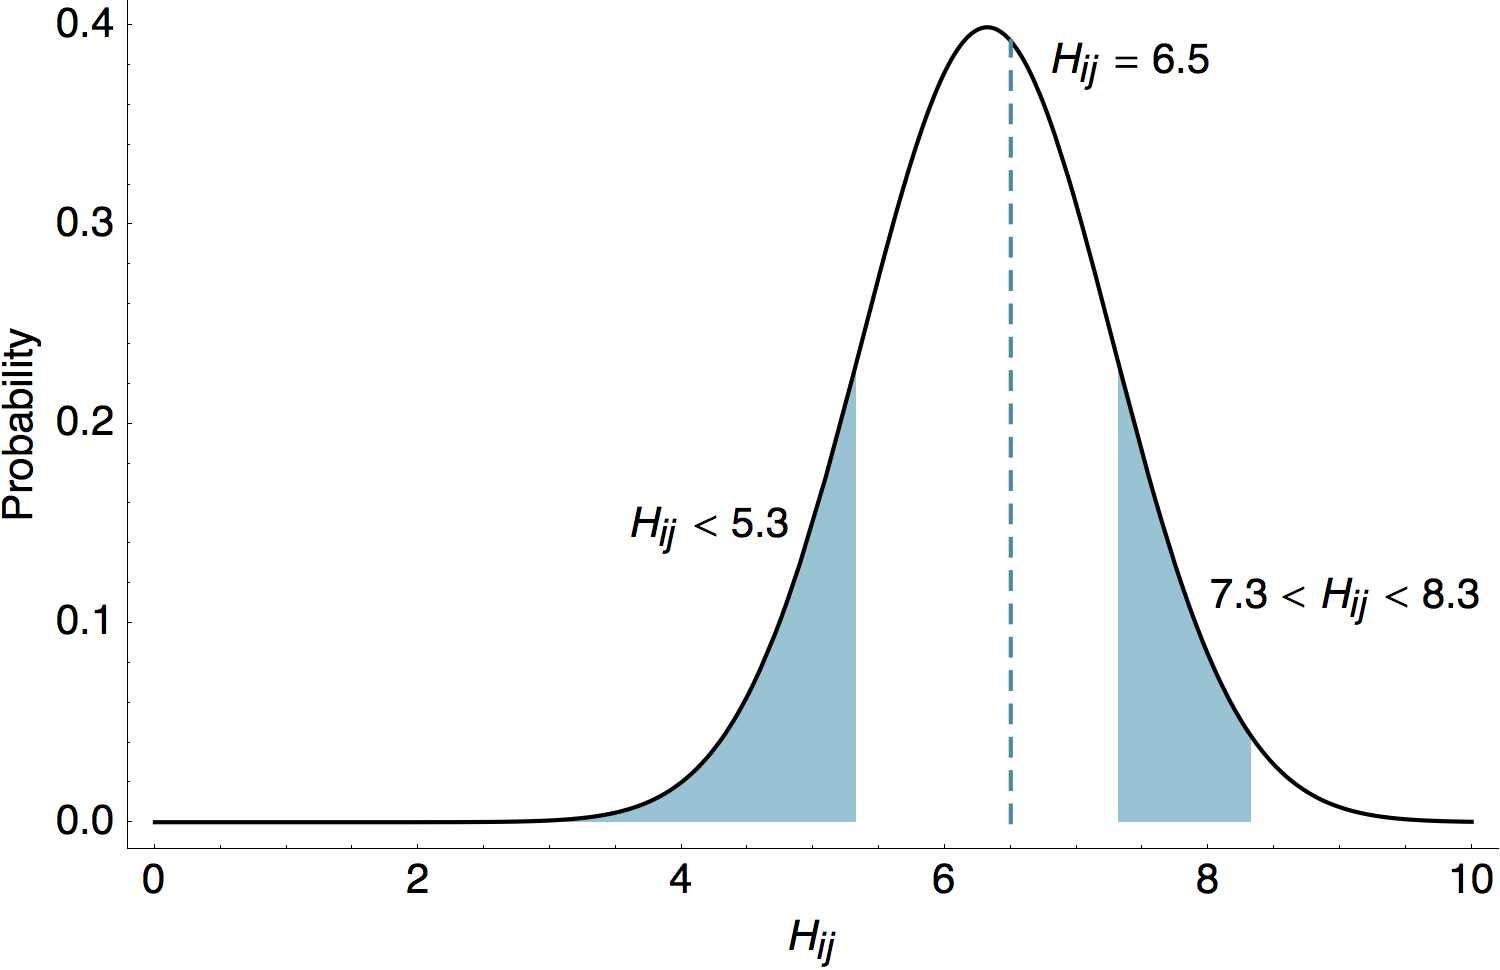
\includegraphics[width=0.6\textwidth]{figures/hij_likelihood}
	\caption{\textbf{Likelihood of HI titers in the BMDS model.} 
	Here we show the likelihoods of observing three different outcomes given $\delta_{ij} = 4$, $\mdssd = 0.95$ and $S_j = \mathrm{log}_2 1280 = 10.32$.  
	The likelihood of observing a threshold titer of `$<$40' is equal to the lower tail of the probability density function $\threshold(5.32) = 0.146$.
	The likelihood of observing a point measurement with an exact inhibiting titer of `90.5' is equal to the density function $\point(6.5) = 0.413$.
	The likelihood of observing an interval measurement with an inhibiting titer somewhere between `160' and `320' is equal to $\interval(7.32) = 0.129.$
	} 
	\label{hij_likelihood} 
\end{figure}

We calculate the overall likelihood by multiplying probabilities of individual measurements
\begin{equation} 
	L(\mathbf{X},\mathbf{Y}) = \prod_{(i,j) \in \cal I} f(H_{ij}),
\end{equation}
using probability functions $\point$, $\threshold$ and $\interval$ as appropriate.
We assume that the prior precision $1/\mdssd^2$ follows a diffuse $\mbox{Gamma}(a, b)$ distribution with $a=0.001$ and $b=0.001$, and we start by assuming a diffuse normal prior $\mathrm{Normal}(\mu,\Sigma)$ over virus and sera locations $\mathbf{X}$ and $\mathbf{Y}$, with $\mu = \twomatrix{0}{0}$ and $\Sigma = \fourmatrix{10,000}{0}{0}{10,000}$ for $P=2$.

We integrate over uncertainty using the Markov chain Monte Carlo (MCMC) procedures implemented in the phylogenetic package BEAST \cite{BEAST,BEAST17}.
Metropolis-Hastings proposals include moves to individual virus and serum locations $X_i$ and $Y_j$, scaling of the entire set of virus and serum locations $\mathbf{X}$ and $\mathbf{Y}$ and scaling $\mdssd$.

\subsection*{Incorporating virus and serum effects}

The preceding model represents immunological distance as a drop in titer against the most reactive comparison for a particular serum.  
Here, we relax this assumption and treat the maximum reactivity of a sera as a random variable.
In this case, $H_{ij}$ still follows equation \ref{hij} with expectation $S_j - \delta_{ij}$, but the vector of `serum effects' $\mathbf{S}$ is estimated rather than fixed.
We assume that $S_j$ values are hierarchically distributed according to a normal distribution.
The mean and variance of this distribution is taken from the empirical mean and empirical variance of the set of maximum titers across sera $\{ \max ( H_{1j},\ldots,H_{\vn j} ) : j = 1,\ldots,\sn \}$.
This formulation assumes that particular sera are more reactive in general than other sera.

Additionally, we follow the same logic and assume that particular virus isolates are more reactive in general than other virus isolates.
With virus reactivity included, the expectation of $H_{ij}$ becomes $(V_i+S_j)/2 - \delta_{ij}$ and the vector of `virus effects' $V_i$ for $i = 1,\ldots, \vn$ is estimated in an analogous hierarchical fashion, with $\mathbf{V}$ normally distributed with mean and variance equal to the empirical mean and variance of the set of maximum titers across viruses $\{ \max ( H_{i1},\ldots,H_{i \sn} ) : i = 1,\ldots,\vn \}$.

With these effects included, Metropolis-Hastings proposals additionally incorporate moves to individual serum effects $S_j$ and virus effects $V_i$.

\subsection*{Antigenic drift prior}

As presented, virus and serum locations $\mathbf{X}$ and $\mathbf{Y}$ accurately characterize antigenic distances between virus strains based on titers from pairwise HI assays.
However, these distances represent only a local description of antigenic space and do not provide a global picture.
An example of this phenomena is shown in Figure~\ref{schematic_map}.
In this case it is impossible to determine from the HI data at hand whether the blue and yellow viruses are antigenically similar or antigenically divergent. 
This presents an issue of model identifiability; multiple antigenic maps give the same likelihood of observing the serological data.
In order to achieve more interpretable antigenic locations we impose a weak prior on global locations.
In influenza, it's clear that antigenic distance between strains increases with time \cite{Smith04,Cai10}.
To capture this, we replace the diffuse normal prior on virus locations with a prior where virus locations follow a normal distribution $\mathrm{Normal}(\mu,\Sigma)$ in which the expectation of the first antigenic dimension increases with date of virus sampling.
Here, $\mu = \twomatrix{\beta \, y_i}{0}$ and $\Sigma = \fourmatrix{\driftsd^2}{0}{0}{\driftsd^2}$ for $P=2$, where $y_i$ is the difference in time between virus $i$ and the earliest sampled virus.
Thus, this model assumes that the virus population drifts in a line across the antigenic map at rate $\beta$.
The parameter $\driftsd$ determines the breadth of the virus population cloud at each point in time.
We assume that both the prior slope $\beta$ and the prior precision $1/\driftsd^2$ follow a diffuse $\mbox{Gamma}(a, b)$ distribution with $a=0.001$ and $b=0.001$.
We further introduce Metropolis-Hastings proposals that scale $\beta$ and $\driftsd$.

%%% schematic_map %%%
\begin{figure}[tb]
	\centering		
	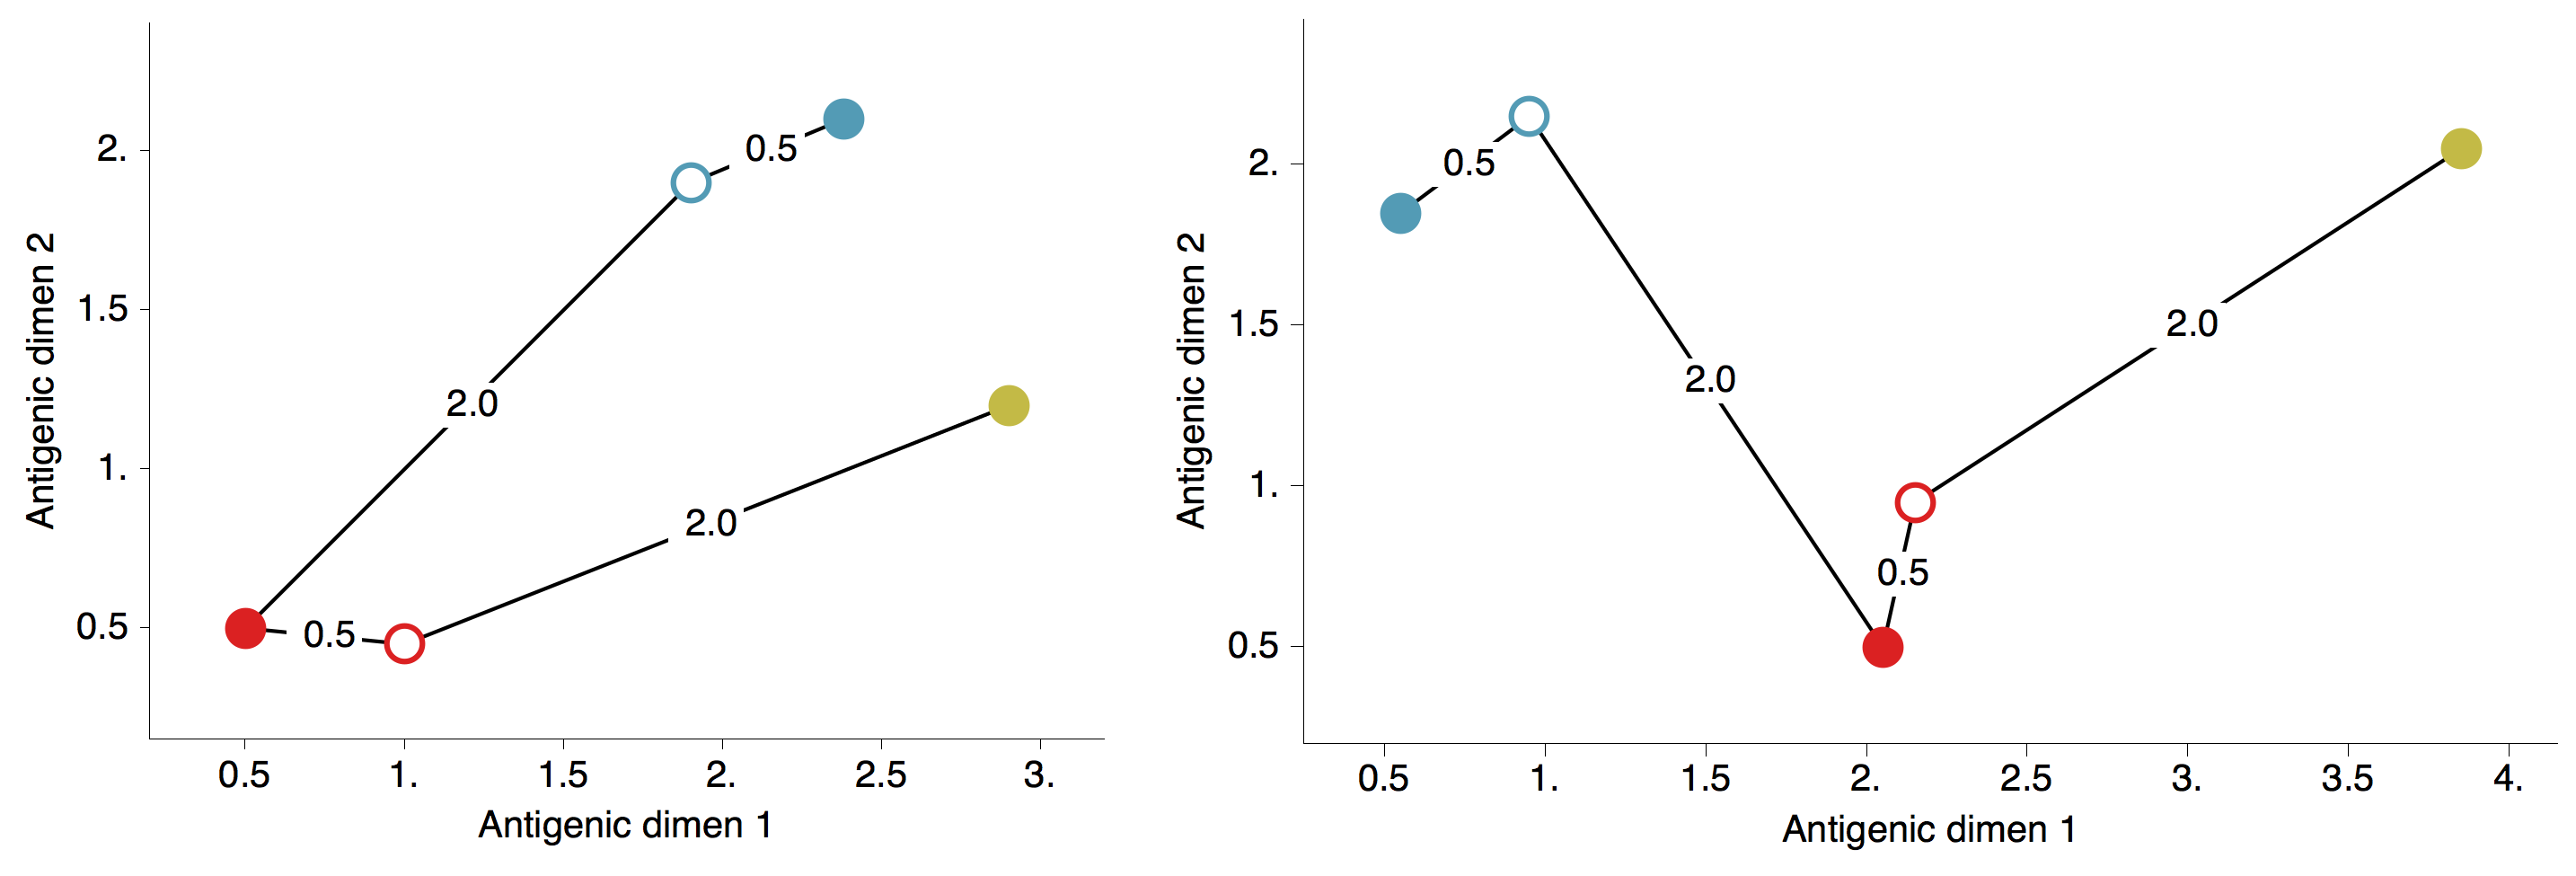
\includegraphics[width=0.95\textwidth]{figures/schematic_map}
	\caption{\textbf{Schematic antigenic map with three viruses and two sera.} 
	Virus 1 is shown in blue, virus 2 is shown in red and virus 3 is shown in yellow.
	Virus isolates are represented by filled circles, sera raised against viruses are shown as open circles and map distances $\delta_{ij}$ are shown as solid lines connecting viruses and sera.
	Sera from virus 1 is compared against viruses 1 and 2, while sera from virus 2 is compared against viruses 1 and 3.
	Left and right panels represent cartographic models that would give equal likelihoods of a given set of serological data $\{H_{11},H_{21},H_{22},H_{32}\}$.
	} 
	\label{schematic_map} 
\end{figure}

\subsection*{Diffusion model of antigenic evolution}

We simultaneously model antigenic locations and genetic relatedness by assuming that viruses diffuse across the antigenic map according to a Brownian motion process \cite{Lemey10}.
To do this, we incorporate a prior on virus locations according to the evolutionary process
\begin{equation}
	(X_1,\ldots,X_n) \sim \mbox{Evolutionary Brownian Process}(\tree, \diffusionsd),
\end{equation}
where $\tree$ is a phylogeny specifying tree topology and branch lengths and $\diffusionsd$ is the volatility parameter of the Brownian motion,  set to have equal variance in each antigenic dimension and no correlation across dimensions.
Thus, viruses which are genetically similar are induced to have prior locations close to one another on the antigenic map.
The phylogenetic tree $\tree$ is estimated using sequence data for viruses $1,\ldots,\vn$ according to well established methods implemented in the software package BEAST \cite{BEAST, BEAST17}.
The volatility parameter $\diffusionsd$ is estimated jointly from the genetic and antigenic data.
Parameter $\diffusionsd$ is assumed to follow a diffuse $\mbox{Gamma}(a, b)$ distribution with $a=0.001$ and $b=0.001$.
Metropolis-Hastings proposals scale $\diffusionsd$.
The probability of observing virus locations $p(\mathbf{X}|\tree,\diffusionsd)$ is determined through analytical integration across internal states following the methods introduced in \cite{Lemey10}.
Thus, under the full model, the posterior probability of observing virus and serum locations given immunological data and phylogeny is factored
\begin{equation}
	p(\mathbf{X},\mathbf{Y} | \mathbf{H},\tree) = \frac{ p(\mathbf{H}|\mathbf{X},\mathbf{Y},\mathbf{S},\mathbf{V}, \mdssd) \; 
	p(\mathbf{X} | \beta, \driftsd) \;
	p(\mathbf{X} | \tree, \diffusionsd) \; 
	p(\mathbf{Y},\mathbf{S},\mathbf{V},\mdssd,\beta,\driftsd,\diffusionsd)}{ p(\mathbf{H}) }.
\end{equation}

\subsection*{Genetic, antigenic and surveillance data}

We compiled an antigenic dataset of hemagglutination inhibition (HI) measurements of virus isolates against post-infection ferret sera for influenza A/H3N2 by collecting data from previous publications \cite{Hay01,Smith04,Russell08,Barr10}, NIMR vaccine strain selection reports for 2002 and 2008--2012 \cite{NIMR02,NIMRMarch08,NIMRFeb09,NIMRFeb10,NIMRSep10,NIMRSep11,NIMRFeb12} and the Feb 2011 VRBPAC report \cite{Cox11FDA}.
We queried the Influenza Research Database \cite{IRD} and the EpiFlu Database \cite{GISAID} for HA nucleotide sequences by matching strain names, e.g.\ A/HongKong/1/1968, and only strains for which sequence was present was retained.
If a strain had multiple sequences in the databases we preferentially kept the IRD sequence and preferentially kept the longest sequence in IRD. 
Sequences were aligned using MUSCLE v3.7 under default parameters \cite{MUSCLE}.
This dataset had 2051 influenza isolates (present as either virus or serum in HI comparisons) dating from 1968 to 2011. 
However, the majority of isolates were present from 2002 to 2007. 
Because we are interested in longer-term antigenic evolution, we subsampled the data to have at most 20 virus isolates per year, preferentially keeping those isolates with more antigenic comparisons. 
We then kept only those serum isolates that are relatively informative to the antigenic placement of viruses, dropping serum isolates that are compared to 4 or fewer different virus isolates.
This censoring left 429 virus isolates, 519 serum isolates and 10,097 HI measurements. 

Antigenic data for influenza A/H1N1 was collected from previous publications \cite{Kendal78,Webster79,Nakajima79,Nakajima81,Chakraverty82,Pereira82,Chakraverty86,Cox83,Daniels85,Raymond86,Stevens87,Donatelli93,Hay01,Daum02,McDonald07,Barr10} and NIMR vaccine strain selection reports for 2002--2010 \cite{NIMR02,NIMR03,NIMR04,NIMRFeb05,NIMRSep05,NIMRMarch06,NIMRSep06,NIMRMarch07,NIMRSep07,NIMRMarch08,NIMRSep08,NIMRFeb09,NIMRFeb10}.
The same procedure was followed as was followed for H3N2 to match sequence data and to subsample antigenic comparisons.
This procedure yielded 124 virus isolates, 77 serum isolates and 1882 HI measurements over the course of 1977 to 2009.

Antigenic comparisons for influenza B/Victoria were collated from previous publications \cite{Rota90, Hay01, Muyanga01, Shaw02, Ansaldi04, Puzelli04, Xu04, Barr06, Daum06, Lin07} and vaccine strain selection reports for 2002--2012 \cite{AusWHO06, NIMR02, NIMR03, NIMR04, NIMRFeb05, NIMRSep05, NIMRMarch06, NIMRSep06, NIMRMarch07, NIMRSep07, NIMRMarch08, NIMRFeb09, NIMRSep09, NIMRFeb10, NIMRSep10, NIMRFeb11, NIMRSep11, NIMRFeb12}.
Here, the sequence matching and subsampling procedure yielded 179 virus isolates, 70 serum isolates and 2003 HI measurements over the course of 1986 to 2011.

Antigenic comparisons for influenza B/Yamagata were collected from previous publications \cite{Rota90, Kanegae90, Nakajima92, Nerome98, Hay01, Muyanga01, Nakagawa02, Abed03, Ansaldi03, Ansaldi04, Matsuzaki04, Puzelli04, Shaw02, Xu04, Barr06, Daum06, Lin07} and vaccine strain selection reports for 2002--2012 \cite{AusWHO06, NIMR02, NIMR03, NIMR04, NIMRFeb05, NIMRSep05, NIMRMarch06, NIMRSep06, NIMRMarch07, NIMRSep07, NIMRMarch08, NIMRFeb09, NIMRSep09, NIMRFeb10, NIMRSep10, NIMRFeb11, NIMRSep11, NIMRFeb12}.
For B/Yamagata, the matching and subsampling procedure resulted in 174 virus isolates, 69 serum isolates and 1962 HI measurements over the course of 1987 to 2011.

Surveillance data was obtained from the Centers of Disease Control and Prevention FluView Influenza Reports from the yearly summaries of influenza seasons 1997--1998 to 2010--2011 \cite{CDCReports}.
As an example, one report states ``collaborating laboratories in the United States tested 195,744 respiratory specimens for influenza viruses, 27,682 (14\%) of which were positive. Of these, 18,175 (66\%) were positive for influenza A viruses, and 9,507 (34\%) were positive for influenza B viruses. Of the 18,175 specimens positive for influenza A viruses, 7,631 (42\%) were subtyped; 6,762 (87\%) of these were seasonal influenza A (H1N1) viruses, and 869 (13\%) were influenza A (H3N2) viruses.''
In this case, we estimate the relative proportion of A/H3N2 of the four clades as $0.66 \times 0.13 = 0.09$.
Similar calculations were performed for A/H1N1, B/Vic and B/Yam.

\subsection*{Implementation considerations}

There were a couple of issues we encountered in applying the BMDS model to HI data from A/H3N2, A/H1N1, B/Vic and B/Yam.
The first issue lay in summarizing the posterior distribution of virus and serum locations.
Although our MCMC procedure samples from the posterior, sampled virus and serum locations represent only relative quantities, and because of this, over the course of the MCMC virus locations may shift dramatically.
Our `antigenic drift prior' removes much of this issue, orienting the antigenic map along dimension 1 and fixing it to begin at $\{0,0\}$.
However, local isometries are often still a problem.
For example, in A/H3N2 the Beijing/89 cluster may shift back and forth from being above other viruses on dimension 2 to being below other viruses on dimension 2.
These isometries may be local, i.e.\ Beijing/89 and Beijing/92 may flip while leaving Texas/77 in place.
Consequently, it is difficult to fully align MCMC samples using Procrustes analysis.
Here, we take a simple approach and sample a single MCMC step and visualize the antigenic locations at this state (Figures~\ref{map}, Figure~\ref{drift}).
Then, for quantities of interest, like rate of antigenic drift and rate of diffusion at different points along the phylogeny, we calculate this quantity across MCMC samples to yield an expectation and a credible interval.

Running the fully parameterized model including the phylogenetic diffusion prior resulted a pathological outcome in which all virus and serum locations are compressed into a single point, diffusion volatility $\diffusionsd$ is tends toward zero and MDS variance $\mdssd^2$ tends towards infinity.
In this case, $p(\mathbf{H}|\mathbf{X},\mathbf{Y},\mathbf{S},\mathbf{V}, \mdssd)$ is reduced, but $p(\mathbf{X} | \tree, \diffusionsd)$ becomes very large, yielding a greater overall posterior probability.
To avoid this problematic outcome we conducted a two stage analysis.
We first estimated values of $\mdssd$, $\beta$ and $\driftsd$ using HI data alone, and then held these values constant in a subsequent analysis that included the phylogenetic diffusion prior.

Phylogenetic trees were sampled for A/H3N2, A/H1N1, B/Vic and B/Yam using BEAST \cite{BEAST} and incorporated the SRD06 nucleotide substitution model \cite{Shapiro06}, a coalescent demographic model with constant effective population size and a strict molecular clock across branches.
MCMC was run for 60 million steps and trees were sampled every 50,000 steps after allowing a burn-in of 10 million steps, yielding a total sample of 2000 trees.
These trees were treated as a discrete set of possibilities when subsequently sampled in the BMDS analysis.

MCMC was used to sample virus locations $\mathbf{X}$, serum locations $\mathbf{Y}$, virus effects $\mathbf{V}$, serum effects $\mathbf{S}$, MDS precision $1/\mdssd^2$, antigenic drift rate $\beta$, population variance $\driftsd^2$, diffusion volatility $\diffusionsd$ and phylogenetic tree $\tree$.
MCMC chains were run for 500 million steps and parameter values sampled every 200,000 steps after a burn-in of 100 million steps, yielding a total of 2000 MCMC samples.

\subsection*{Availability}

Source code implementing the cartographic models has been made fully available as part of the software package BEAST \cite{BEAST, BEAST17}, and can be downloaded from its Google code repository (http://code.google.com/p/beast-mcmc/).
Antigenic, genetic and surveillance data is available as supplemental information \tbc{PREPARE}.
Also included as supplemental information are XML control files to load antigenic and phylogenetic data into BEAST and perform cartographic analyses \tbc{PREPARE}.

%%% ACKNOWLEDGMENTS %%%
\subsection*{Acknowledgments} 

We thank Richard Reeve, Dan Haydon, and Simon Frost for insights on antigenic modeling and MDS.
We thank John McCauley for making NIMR vaccine strain selection reports publicly available.
We acknowledge the laboratories that provided sequences to EpiFlu database: Centers for Disease Control and Prevention (USA), Chinese Center of Disease Prevention and Control, Hospital Clinic of Barcelona, National Institute of Hygiene of Morocco, National Institute of Infectious Diseases (Japan), National Institute for Medical Research (UK), Norwegian Institute of Public Health, Swedish Institute for Infectious Disease Control, Victorian Infectious Diseases Reference Laboratory (Australia).

%%% AUTHOR CONTRIBUTIONS %%%
\subsection*{Author contributions} 

AR, MAS, TB, and PL conceived the study.
TB, GD, CR, DS and AR gathered antigenic and genetic data.
AR, MAS, TB, and PL designed statistical phylogenetic procedures.
TB performed the analysis.
TB, MAS, AR wrote the paper.

%%% FUNDING %%%
\subsection*{Funding} 

TB is supported by the Royal Society.

%%% REFERENCES %%%
\bibliographystyle{plos}
\bibliography{flux}

%\pagebreak

%\setcounter{figure}{0}
%\setcounter{table}{0}
%\setcounter{page}{1}
%\renewcommand{\thefigure}{S\arabic{figure}}
%\renewcommand{\thetable}{S\arabic{table}}
%\renewcommand{\thepage}{S\arabic{page}}

%%% SUPPORTING INFORMATION %%%
%\section*{Supporting Information}


\end{document}
